
% Template for Seminar Papers
% Research Group for Parallel Computing
% TU Wien

% Copyright (C) 2015-2018
% Sascha Hunold <hunold@par.tuwien.ac.at>
% version 1.2.0

\documentclass[DIV12,a4paper]{scrartcl}

\usepackage[utf8]{inputenc}
\usepackage[T1]{fontenc}

%\usepackage{fixltx2e}
\usepackage{amsmath}
\usepackage{amssymb}
\usepackage{amsthm}
\usepackage{IEEEtrantools}
\usepackage[algoruled]{algorithm2e}
\usepackage{microtype}
\usepackage{enumitem}
\usepackage{booktabs}
% Issues warnings when best practices in writing LaTeX documents are violated.
\usepackage{nag}
\usepackage{xspace}
\usepackage{graphicx}
% need this for DOI (or use biber/biblatex)
\usepackage[square,numbers]{natbib}
\usepackage{bibentry}
\usepackage[hidelinks]{hyperref}
\usepackage[binary-units]{siunitx}
\nobibliography*

\DeclareMathOperator*{\argmin}{\arg\!\min}
\DeclareMathOperator*{\argmax}{\arg\!\max}
\DeclareMathOperator*{\lexmin}{\lex\!\min}
\DeclareMathOperator*{\lexmax}{\lex\!\max}

%%%%%%%%%%%%%%%%%%%%%%%%%%%%%%%%%%%
% ONLY CHANGE THE FOLLOWING MACROS

% your name
\newcommand{\studname}{Aleksandr Lisianoi}

% your matrikel
\newcommand{\studmatrikel}{01527346}

% name of seminar
\newcommand{\seminarname}{Scheduling Algorithms for Clusters, Distributed Systems, and Multi-core Nodes}

% title of your seminar paper (is usually title of the paper)
\newcommand{\seminartitle}{Scheduling Jobs across Geo-Distributed Datacenters with Max-Min Fairness}

% date when you hand in seminar paper
\newcommand{\spdate}{\today}

% uncomment your choice
%\newcommand{\sptopic}{Seminar aus Programmiersprachen}
\newcommand{\sptopic}{Seminar aus Algorithmik}
%\newcommand{\sptopic}{Seminar aus Software Engineering}
%\newcommand{\sptopic}{Seminar aus Theoretischer Informatik}
%\newcommand{\sptopic}{Seminar aus Technischer Informatik}

% who is supervising
\newcommand{\spbetreuer}{Ass.Prof. Dr. Sascha Hunold}
%\newcommand{\spbetreuer}{Prof. Dr. Jesper Larsson Träff}

% YOU SHOULD NOT NEED TO CHANGE THE REMAINING FILE
%%%%%%%%%%%%%%%%%%%%%%%%%%%%%%%%%%%

\graphicspath{{graphics/}}


\begin{document}
\hypersetup{pageanchor=false}

% !TEX root = template.tex

\pagestyle{empty}

\begin{titlepage}
\begin{center}

\includegraphics[scale=1]{TU_INF_Logo_gray}
\hfill

\includegraphics[width=1.7cm]{final-logo-par}

\end{center}

\vspace*{1cm}

\begin{center}

\begin{Large}
Institute of Computer Engineering \\
Research division ``Parallel Computing'' (E191-4)
\end{Large}

\vspace*{1cm}

\begin{Huge}
\textbf{Seminararbeit}\\
\end{Huge}

\vspace*{1cm}

\begin{Large}
für ein \\
\sptopic{} \\
``\seminarname{}'' 
\end{Large}


\vspace*{2cm}

\begin{Large}
\textbf{``\seminartitle{}''}
\end{Large}

\vspace*{2cm}

\begin{Large}
\studname \\
Matrikelnummer: \studmatrikel\\[2cm]

Betreuer: \spbetreuer

\vspace*{2cm}
\spdate \\

\end{Large}
\end{center}

\end{titlepage}


\cleardoublepage


\section*{Main Literature Sources}

\begin{NoHyper}
The following seminar report is based on the following research articles:
% !TEX root = template.tex

% CHANGE THIS LIST ACCORDINGLY
% these are the papers that you received for your topic
% this list should not include the other papers that you are referencing, those should go to the bibliography

\begin{itemize}
  \item \bibentry{Chen2017}
\end{itemize}

\end{NoHyper}

\clearpage

% !TEX root = template.tex

\section*{Erkl\"arung zur Verfassung der Arbeit}

\vspace*{3ex}

\noindent
Hiermit erkl\"are ich, dass ich diese Arbeit selbst\"andig verfasst habe, dass ich die verwendeten Quellen und Hilfsmittel vollst\"andig angegeben habe und dass ich die Stellen der Arbeit -- einschließlich Tabellen, Karten und Abbildungen --, die anderen Werken oder dem Internet im Wortlaut oder dem Sinn nach entnommen sind, auf jeden Fall unter Angabe der Quelle als Entlehnung kenntlich gemacht habe.\\[5ex]

\noindent
\rule{8cm}{.5pt} \\
Wien, \spdate \\
\studname


\clearpage

\hypersetup{pageanchor=true}
\tableofcontents

\cleardoublepage

\pagestyle{plain}

\setcounter{page}{1}

% !TEX root = template.tex

\section{Introduction}

Here goes the introduction. We also cite the nice book by \citet{Pinedo:2012}.
This might be a book with interesting topics, but concurrent time-stamping has also been addressed before~\cite{Dolev97}.
In this work, \citet{Dolev97} presented the first bounded implementation of a concurrent time-stamp system.


\section{Algorithm X}

Table~\ref{tab:related_algorithms} shows a summary of related algorithms.

\begin{table}[h]
\centering
\captionabove{Related algorithms and their complexity.}
\label{tab:related_algorithms}
\begin{tabular}{ll}
\toprule 
algorithm & complexity \\
\midrule
algorithm Y & $\mathcal{O}(n)$ \\
algorithm Z & $\mathcal{O}(n \log{n} )$ \\
\bottomrule
\end{tabular}
\end{table}

\section{Evaluation of Algorithm X}


\subsection{Evaluating the Running Time of Algorithm X}

The run-time of our algorithm is shown in Figure~\ref{fig:runtime}.
We can observe that the run-time of our algorithm increases linearly with the message size.
Since we target a system with a run-time of less than \SI{10}{\second}, the maximum message size should be \SI{128}{\byte}.

\begin{figure}[h]
\centering
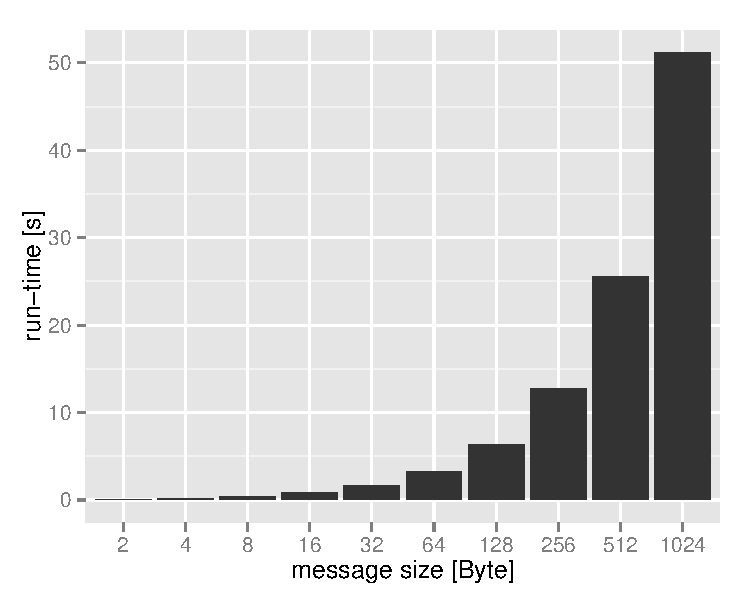
\includegraphics[width=.5\linewidth]{figures/runtime}
\caption{Run-time of algorithm X on machine Y.}
\label{fig:runtime}
\end{figure}

\subsection{Evaluating the Space Requirements of Algorithm X}

Now, we investigate the space requirements of the algorithms listed in Table~\ref{tab:related_algorithms}.


\section{Summary}
We summary the contribution of the papers and this seminar paper.


\cleardoublepage
% Add a bibliography
\bibliographystyle{plainnat}
\bibliography{myreferences}

\end{document}
